\documentclass[12pt]{article}
\setlength{\textwidth}{17cm}
\setlength{\textheight}{24cm}
\setlength{\topmargin}{-2cm}
\setlength{\footskip}{1cm}
\setlength{\evensidemargin}{0cm}
\setlength{\oddsidemargin}{0cm}
\setlength{\parindent}{0cm}

\usepackage{allrunes}
\usepackage{amsmath}
\usepackage[magyar]{babel}
\usepackage[T1]{fontenc}
\usepackage[utf8]{inputenc}
\usepackage{fixltx2e}
\usepackage{multirow}

\usepackage[hyphens]{url}
\usepackage[unicode,colorlinks=true,breaklinks]{hyperref}
%\usepackage[dvips]{hyperref}
%should display links, but it does not work with \H accent
%and formulas in section titles

\hypersetup{colorlinks,linkcolor=blue,urlcolor=magenta,citecolor=magenta}
%Breaks long url`s in text, while keeping it one link:

\usepackage{amsfonts}
\usepackage{amsthm}
\usepackage{amssymb}


\theoremstyle{plain}
\usepackage{graphicx}

%\usepackage{gensymb}
\usepackage{float}

% For bra-ket notation
\usepackage{braket}

%% New commands
\newcommand{\dd}{\textrm{d}}

%% Pauli matrices
\newcommand{\sigx}{\sigma_x}
\newcommand{\sigy}{\sigma_y}
\newcommand{\sigz}{\sigma_z}

\newcommand{\paulix}{
    \left( \begin{array}{cc}
        0 & 1 \\
        1 & 0
    \end{array}
    \right)
}

\newcommand{\pauliy}{
    \left( \begin{array}{cc}
        0 & -i \\
        i & 0
    \end{array}
    \right)
}

\newcommand{\pauliz}{
    \left( \begin{array}{cc}
        1 & 0 \\
        0 & -1
    \end{array}
    \right)
}


\begin{document}
\title{5. tétel}
\author{Furuglyás Kristóf}

\maketitle


\newpage
\begin{abstract}
    Fraktáldimenzió, önhasonló matematikai fraktálok, természetben előforduló fraktálok, sejtautomaták.
\end{abstract}

\section{Fraktáldimenzió}
Mindennapi objektumoknál megfigyelhető, hogy ha egyre kisebb skálán vizsgáljuk őket, az egyes tulajdonságaik konvergálnak egy adott értékhez. Fraktálok esetében azonban a kisebb felbontás nem eredményez konvergenciát; \textbf{a fraktálok határai} ugyanis végtelenül "gyűröttek" vagy "szakadásosak", azaz \textbf{nem-differenciálhatóak}. Továbbá, a fraktálok másik fontos tulajdonsága, hogy \textbf{önhasonlók} -- azaz különböző nagyítás mellett nézve ugyanazt az alakzatot látjuk kibontakozni. A természetben előforduló fraktálok például a \textbf{szigetek partvonalai vagy a hegyek felszíne}. Előfordulhatnak még \textbf{növekedésből származó fraktálok} is, mint például az a \textbf{növények gyökérzete vagy épp a keringési rendszer}. Ilyenkor az elégazó struktúrák valamilyen \textbf{növekedési instabilitás} váltja ki. \\

Megmérve bármilyen $d$ dimenziós test a térfogatát különböző $l$ oldalhosszúságú szintén $d$ dimenziós (tehát $l^d$ térfogatú) kockákkal, és feltételezve, hogy ekkor a lefedéshez szükséges kockák száma $N \left( l \right)$, a test téfogata: 

\begin{equation}
V \left( l \right) =  N \left( l \right) \cdot l^d.
\end{equation}

Hétköznapi objektumoknál ha $l \rightarrow 0$, akkor $V \left(l \right)$ gyorsan konvergál egy adott értékhez. Azonban \textbf{fraktálok} esetében ha $l \rightarrow 0$, akkor $\mathbf{V \left(l \right) \rightarrow 0}$! Ugyanakkor ezzel egyidőben a $d-1$ dimenziós $S \left( l\right)$ \textbf{felszíne pedig divergál}: $\mathbf{ S \left( l \right) \rightarrow \infty}$. \\

A geomatriai (matematikai) fraktálok:
\begin{itemize}
	\item olyan \textbf{önhasonló} geometriával rendelkező formák,
	\item ahol az önhasonlóság \textbf{tetszőleges iteráción keresztül} fennáll, 
	\item és a lefedéshez szükséges $l$ élhosszúságú dobozok $N \left( l \right) $ száma \textbf{nemtriviálisan skálázódik}:
		\begin{equation}
					N \left( l \right) \sim l^{-D},
		\end{equation}
	ahol $D$ egy pozitív, nem egész szám, amely az objektum törtdimenziója, fraktáldimenziója.
\end{itemize}

Az előbbiek alapján a két oldal logaritmusát véve definiálhatjuk a fraktál \textbf{box-counting dimenzióját}:
\begin{equation}
D_B = \lim_{l \rightarrow 0 } \frac{\ln N \left( l\right) }{\ln \left(1/l\right)}.
\end{equation}
Ugyanez érvényes akkor is, \textbf{ha a fraktál növekvő}, és annak lineáris hosszát $L$-lel jelöljük:
\begin{equation}
D_B = \lim_{L \rightarrow \infty } \frac{\ln N \left( L\right) }{\ln L}.
\end{equation}



\begin{figure}[H]
    \begin{center}
    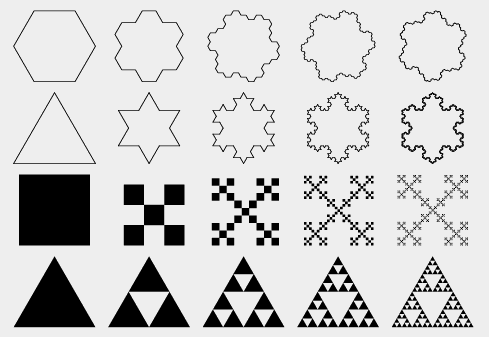
\includegraphics[width=0.5\textwidth]{media/fractal_pelda.png}
    \caption{Példa fraktálokra különböző iterációk után. Lehet látni, hogy változik a térfogat és a felszín aránya. } 
    \label{fig:fractal_peldak}
    \end{center}
\end{figure}

\subsection{Műveletek}

A fraktálokkal, mint matematikai objektumokkal műveleteket is végezhetünk:
\begin{itemize}
	\item \textbf{Projekció}: $d$ dimenziós euklidészi térbe ágyazott $D$ dimenziós fraktált projektálunk egy $d_s$ dimenziós szintér eklidészi altérre:
	\begin{itemize}
		\item ha $d_s>D$, akkor a projekció dimenzió nem változik, $D_p = D$,
		\item ha $d_s<D$, akkor a projekció kitölti a rendelkezésre álló teret, $D_p = d_s$. Tehát $\mathbf{D_p =\max \left(D, d_s\right) }$ .
	\end{itemize}  
	\item \textbf{Metszet I.} : ha vesszük egy $d$ dimenziós euklidészi térbe ágyazott $D$ dimenziós fraktál és egy $d-m$ dimenziós szintén euklidészi tér metszetét, akkor a metszet dimenziója $\mathbf{D_i = D-m}$ lesz.
	\item \textbf{Metszet II.} : két fraktál metszetének dimenzióját a részecskék sűrűségéből tudjuk kiszámolni:
	\begin{itemize}
		\item egy $L$ lineáris hosszúságú szakaszon az $A$ fraktál részecskéinek sűrűsége $\sim \frac{L^{D_A}}{L^d}$, B-nek hasonlóképp,
		\item mivel a két fraktál részecskéinek eloszlása független egymástól, az együttes sűrűség $\sim \frac{L^{D_A}}{L^d} \cdot \frac{L^{D_B}}{L^d}$, az összes részecskét pedig a teljes térre nézzük -- $N_{A \cap B} \left(L \right) \sim \frac{L^{D_A} L^{D_B}}{L^d}$,
		\item tehát a dimenzió leolvasható: $\mathbf{D_{A \cap B} = D_A + D_B - d}$.
	\end{itemize}
	\item \textbf{Unió}: két fraktál uniójának dimenzióját a nagyobbik dimenziójú fraktál fogja megadni, azaz $\mathbf{D_{A\cup B} = \max \left( D_A, D_B \right) }$.
	\item \textbf{Szorzat}: két fraktál szorzatának dimenziója a fraktálok dimenziójának összege, azaz $\mathbf{D_{AB} = D_A + D_B}$.

\end{itemize}

\subsection{Típusok}

\paragraph{Determinisztikus fraktál}
Egy fraktál determinisztikus, ha önhasonló rekurzióval generálódik -- azaz vagy kicseréljük a részeit önmaga lekicsinyített képével vagy önmaga felnagyított képével. Ezekre tökéletes példát mutat a \ref{fig:fractal_peldak}. ábra. Például, ha harmadik sorban egységoldalúnak vesszük az első ábrát és a mellette lévőket felskálázzuk úgy, hogy az egyes négyzetek oldalai rendre egységhosszúak legyenek, akkor egy növekvő fraktált kapunk. Ennek a fraktálnak a lineáris mérete a háromszorosára, kvázi "területe", azaz a lefedéshez szükséges négyzetek száma pedig az ötszörösére nő. Ezek alapján a fraktál dimenziója:

\begin{equation}
D = \lim_{L \rightarrow \infty } \frac{\ln N \left( L\right) }{\ln L} = \lim_{k \rightarrow \infty} \frac{ \ln \left( 5 ^k\right) }{ \ln \left( 3^k\right)} = \frac{\ln 5}{ \ln 3} = 1.465\dots
\end{equation}

\begin{figure}[H]
    \begin{center}
    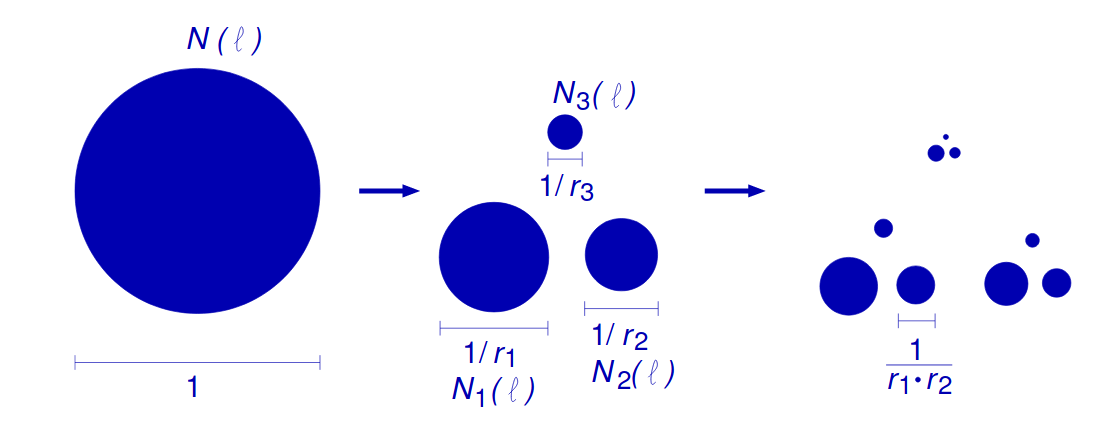
\includegraphics[width=0.5\textwidth]{media/fractal_non_uni.png}
    \caption{Példa non-uniform fraktálra. } 
    \label{fig:fractal_non_uni}
    \end{center}
\end{figure}

Előfordulhat azonban, hogy nem egyenletes a másolatok nagysága -- lásd \ref{fig:fractal_non_uni}. ábra. Ekkor ha $q$ különböző másolatot készítünk ($r_1, r_2, \dots, r_q$), akkor az összes lefedéshez szükséges négyzet az elsóbb fraktálokból jön: $N \left( l \right) = \sum_{i = 1}^q N_i\left( l\right)$. Az önhasonlóság miatt $ N\left( l\right) = N_i\left( l / r_i\right)$. A fraktál definíciójából jön, hogy $N_i \left( l\right) = N \left( lr_i \right) \sim \left( lr_i \right)^{-D_B}$. Visszahelyettesítve $N \left( l \right) = \sum_{i = 1}^q N_i\left( l\right) =\sum_{i = 1}^q \left( lr_i \right)^{-D_B} \sim l^{-D_B}$, tehát a dimenzióra egy implicit egyenletet kapunk: $\sum_{i_1}^q r_i^{-D_B} = 1$.






\paragraph{Szotochasztikus fraktálok}
Hasonlóképp, mint a determinisztikus fraktáloknál, itt is van egy önhasonló rekurzió, mellyel generálódik a fraktál, azonban ekkor bejön továbbá egy random tényező. Ha a random tényező nem befolyásolja fraktál méretét, csak a struktúráját, akkor a fraktál box-counting dimenziója ugyanaz, mint a determinisztikus esetben -- lásd \ref{fig:stoch_cantor}. ábra.

\begin{figure}[H]
    \begin{center}
    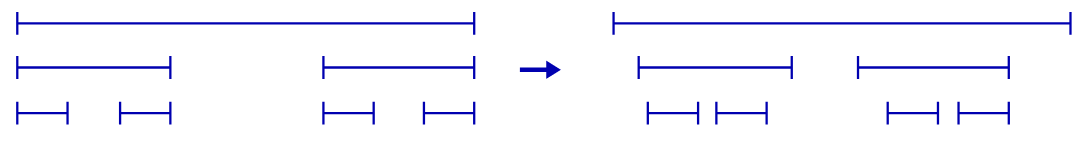
\includegraphics[width=0.5\textwidth]{media/stoch_cantor.png}
    \caption{Sztochasztikus Cantor halmaz. Bal oldalon determinisztikus, jobb oldalon sztochasztikus formában. Észrevehető, hogy a lefedéshez szükséges négyzetek száma $(N \left( l \right))$ nem változik.} 
    \label{fig:stoch_cantor}
    \end{center}
\end{figure}

\paragraph{Random fraktálok}

\begin{figure}[H]
    \begin{center}
    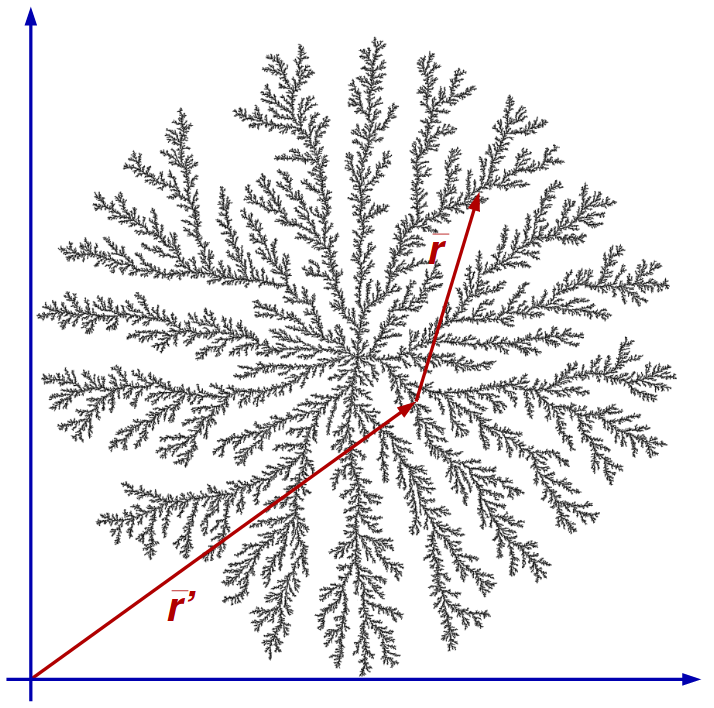
\includegraphics[width=0.5\textwidth]{media/dla_frac.png}
    \caption{Diffúzió-limitált növekedés következtében kialakult random fraktálszerkezet. Ilyen lehet például egy baktériumtelep, vagy elektromos áram elvezetése fában.}
    \label{fig:dla_frac}
    \end{center}
\end{figure}

\begin{figure}[H]
    \begin{center}
    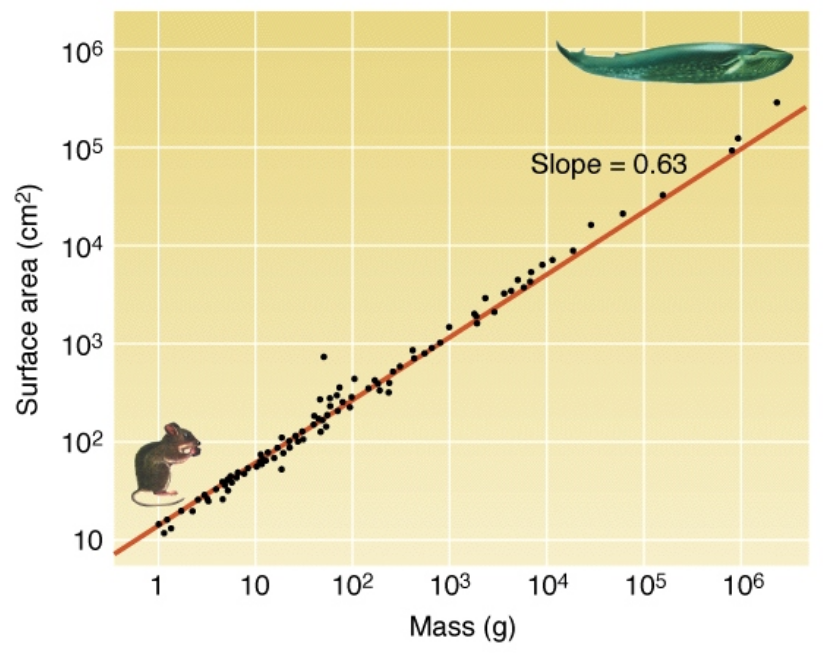
\includegraphics[width=0.5\textwidth]{media/allometry.png}
    \caption{Az állatok tömegének és felületének összefüggése log-log skálán.}
    \label{fig:allometry}
    \end{center}
\end{figure}

A legtöbb, természetben előforduló fraktál ilyen. Ekkor nincsen iterációs szabály, és emiatt a dimenzió kiszámítása is bonyolulttá válhat, ezért célszerűbb a sűrűség-korrelációs függvényt vizsgálni:

\begin{equation}
C\left( \vec{\mathbf{r}} \right) = \frac{1}{V} \sum_{\vec{\mathbf{r'}}} \rho \left(\vec{\mathbf{r + r'}} \right)\rho \left(\vec{\mathbf{r'}} \right),
\end{equation}
ahol $V$ a térfogat, a szumma a tér minden pontjára vonatkozik, a $\rho \left(\vec{\mathbf{r}} \right)$ pedig a sűrűségfüggvény, mely $=1$ ha a $\vec{\mathbf{r}} $ pontban van fraktál és $=0$ egyébként -- \ref{fig:dla_frac}. ábra. A sűrűség-korrelációs függvény izotróp testek esetében csak a sugártól függ, és amíg hétköznapi objektumokra a lépcsőfüggvény, kristályrácsra pedig diszkrét vonalak, addig fraktáloknál skálázódik:

\begin{equation}
C\left(r\right) \sim r^{-\alpha}.
\end{equation}

A skálázódásra példa lehet \href{https://en.wikipedia.org/wiki/Zipf's_law}{Zipf törvénye}, illetve a biológiában az allometria (élőlények tulajdonságia közötti arány). A skálázódásból fakadóan kiszámítható a fraktálhoz szükséges négyzetek száma:

\begin{equation}
N \left( L \right)  \sim \int_0^L C \left( r \right) d^dr \sim L^{d-\alpha},
\end{equation}

melyből leolvasható, hogy $D = d- \alpha$. 

\section{Természetben előforduló fraktálok}

\subsection{Random mozgás}

\subsection{Lévy repülés}

\subsection{Aggregátumok, perkoláció}

\subsection{Diffűzió-limitált növekedés}
\subsubsection{Alapok}
\subsubsection{Kísérletek}
\subsubsection{Szimuláció}
\subsubsection{Fraktáldimenzió}
\subsubsection{Variációk}


\section{Sejtautomaták}








\bibliographystyle{plain}
\bibliography{references}

\end{document}
